%!TEX program = xelatex
\documentclass[UTF8]{article}
\usepackage{graphicx}
\usepackage{setspace}
% \usepackage{ctex}
\usepackage{amsmath}
\usepackage{geometry}
\geometry{a4paper,left=2cm,right=2cm,top=1cm,bottom=1cm}
\setstretch{1.5}
\title{Summary}
\author{Dis\cdot count}
% \date{Feb 2019}
\begin{document}

\maketitle{}
At first, we will apply the cooperative theory on the machine schedule problem, and put it as a simple example to show our result.

\section{Assumption}
Let $N={1,2,\ldots,n}$ be a set of n players. The number of machines is $m$ and the setup cost is $t_0$.
For convenience of expression, we set the processing times $t_i, i\in N$ satisfy $t_1<t_2<\cdots<t_n$.

\section{Example}
In this example, the grand coalition contains four players, whose processing times on the identical parallel machine are $t_1=2,t_2=3,t_3=4,t_4=5$ respectively. And the machine setup cost is $t_0=9.5$.
So we can conclude that the optimum solution is the grand coalition needs two machines, and additive $0.75$ subsidy. When we increase the setup cost from 9.5 to 13, the number of machine will decrease from 2 to 1.

\section{Conclusion}
Now we extend the number of players to a more complex case, that is we will set the number of players to $n$.
In this situation, the interval size of setup cost can be calculated when $t_i$ is known. And we can obtain that under what circumstances the machine number will change. We set the different intervals where the number of machines remain unchanged as $I_i$ respectively. The extreme points of these intervals are recorded as $S_i$ respectively. Specially, $S_1$ denotes the extreme point of the whole interval, which means the value of setup cost when subsidy equals zero.


We will demonstrate the three parts of the graph.




Because the costs of all the exponential coalitions can be easily got by the SPT rules, we have Lemma1

\section{Lemma1}
The value at the extreme points of the sub-intervals $I_i$ can be calculated with processing times $t_i$ by comparing the costs of the grand coalitions where all the players use two adjacent numbers of machines.

According to the above lemma1, we can obtain all the extreme points of the sub-intervals, i.e., the number of using machines decreases by one when the setup cost equals $S_i$.

\section{Lemma2}
The characteristic function must be supermodular, then we can get the positive setupcost when the machine number changes.



\section{Corollary1}
According to the foregoing description, we have the equation $S_{1}=S_{2}+\cdots+S_{n}=\sum_{i=2}^n S_i$.

With corollary1, we obtain all the breakpoints during the interval of the setup cost where the machine number changes and the subsidy is $0$. Then we'll focus on the specific property of subsidy.

\section{Corollary2}
The least absolute value of the slope during all the intervals is $\frac{1}{n-1}$.
The values of the slope during the sub-intervals are proper fraction. Meanwhile the sum of numerator and denominator is no more than $n$.

\section{Corollary3}
The subsidy is always zero when m is larger than $\frac{n}{2}$. In other words, when the numbers of machine is larger than half of players, the grand coalition don't need any subsidy from the externality.

Until here, we described the main property of the whole figure.
And a diagram of the number of machines and subsidy on setup cost, with its essential features is showed below.

\begin{figure}[h]%%图
	\centering  %插入的图片居中表示
	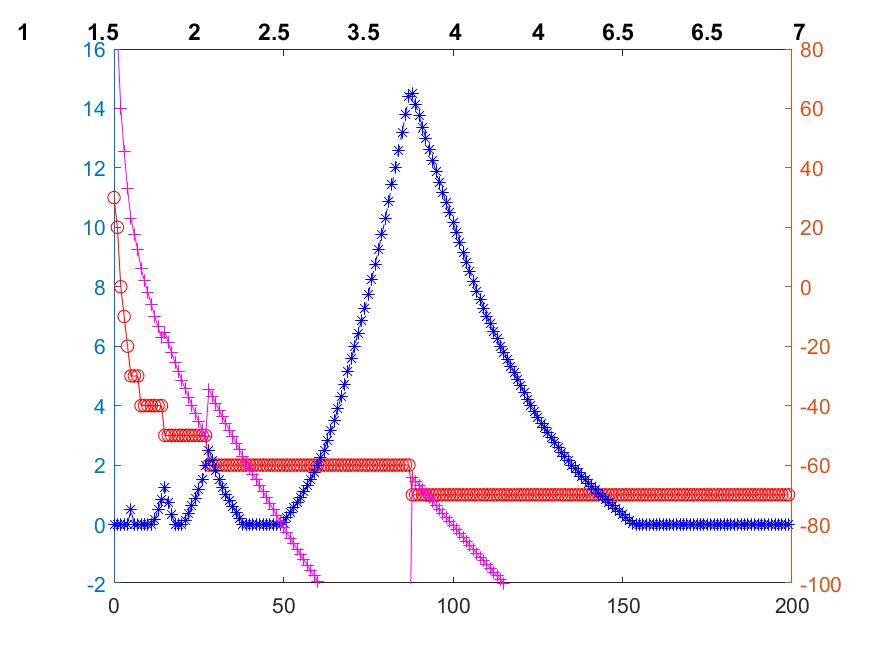
\includegraphics[width=0.8\linewidth]{Figures/Image30}  %插入的图,包括JPG,PNG,PDF,EPS等,放在源文件目录下
	\caption{The number of machines and subsidy on setup cost.}  %图片的名称
	\label{fig:Image11}   %标签,用作引用
\end{figure}

The processing times of all players with the arrangement from small to large are listed on the top of this figure.
The red and blue lines stand for the machine number and subsidy,respectively.
The horizontal ordinate represents setup cost.
The left ordinate represents the value of machine number,while the right represents the value of subsidy.

\section{Proof1}

For convenience of expression, we set the setup cost as $S_{1},S_{2}, \dots ,S_{n}$ at interval points while the number of machine changes.
And $S_{i}$ denotes the setup cost when the machine number changes from $i$ to $i-1$, especially, $S_{1}$ denotes the least setup cost when machine number is $1$ and the corresponding subsidy is $0$.
We have the equality

\begin{displaymath}
  S_{1}=S_{2}+\cdots+S_{n}=\sum_{i=2}^n S_i.
\end{displaymath}

Notice that

\begin{displaymath}
  (n-1) \sum_{s \in S \setminus\{V\} } \rho_s \geq
  \sum_{k\in V}\sum_{s \in S \setminus\{V\}:k \in s} \rho_s = n.
\end{displaymath}

The left side of the inequality means for every $\rho_s$ can appear at most $(n-1)$ times, so we should know that if and only if for every $\rho_s > 0$ appears $n-1$ times the quality holds.That is to say, the coalitions which contains $n-1$ players are all maximally unsatisfied coalitions. Then we have $n \choose n-1$ equalities.
\[
\begin{cases}
 \alpha_1+\alpha_2+ \cdots+\alpha_{n-1} & = x_1 \\
 \alpha_1+\alpha_3+ \cdots+\alpha_n & = x_2 \\
 \quad   \vdots        &\vdots\\
 \alpha_2+\alpha_3+ \cdots+\alpha_n & = x_n.
\end{cases}
\]

Add these $n$ equations together, and we can get

\begin{equation*}
  (n-1)(\alpha_1+\alpha_2+ \cdots+\alpha_n)=\sum_{i=1}^{n}x_i
\end{equation*}

As we know, $x_1,x_2,\dots,x_n$ can be expressed as follows:

\[
\begin{cases}
x_1 = S_0 + (n-1)t_1 + (n-2)t_2 + &\cdots + t_{n-1} \\
x_2 = S_0 + (n-1)t_1 + (n-2)t_3 + &\cdots + t_{n-1} \\
\quad   \vdots        &\vdots\\
x_n = S_0 + (n-1)t_2 + (n-2)t_3 + &\cdots + t_{n}
\end{cases}
\]

According to SPT rule, we can obtain the equality
$c(V)=\alpha_1+\alpha_2+\cdots+\alpha_n=S_0+nt_1+(n-1)t_2+\dots+t_n$.
By replacing $x_1,x_2,\dots,x_n$ together with the expression of $c(V)$, we can get a equality only with $S_0,x_1,x_2,\dots,x_n$.

Finally, we can obtain $S_0 = \sum_{k=1}^n (n-k)t_k$.
\qed

\section{Proof2}



\section{Suppose1}
This one is about how to predict the slope of machine scheduling.




As we konw,




\section{Suppose2}





\end{document}
